%%%%%%%%%%%%%%%%%%%%%%%%%%%%%%%%%%%%%%%%%%%%%%%%%%%%%%%%%%%%%%%%%%%%%%%%
% Preamble
%%%%%%%%%%%%%%%%%%%%%%%%%%%%%%%%%%%%%%%%%%%%%%%%%%%%%%%%%%%%%%%%%%%%%%%%
\documentclass[11pt]{article}
%
% Packages and other includes
% Pagination
\usepackage[letterpaper, margin=0.8in]{geometry}
\usepackage{hyphenat}
\usepackage{multicol,wrapfig}
\hyphenation{Filipp}
%
% Fonts
\usepackage[T1]{fontenc} % best for Western European languages
\usepackage{lmodern} % Latin Modern instead of CM
\usepackage{textcomp} % required to get special symbols
%
% Math
\usepackage{amsmath, amssymb}
\usepackage{braket}
%
% Graphics, floats, tables
\usepackage{graphicx, color, float, array}
%
% Hyperlinks
\usepackage[hidelinks]{hyperref}
%
% Bibliography
\usepackage[style=chem-acs, sorting=none, backend=biber]{biblatex}
\addbibresource{references.bib}
%
% Revision (see Makefile)
%\input{revision.tex}
%
% Definitions and settings
% Paragraph indent and spacing
\setlength{\parskip}{0.4\baselineskip}
\setlength{\parindent}{0in}
%
% Math mode version of "r" column type (requires array package)
\newcolumntype{R}{>{$}r<{$}}
%
% Title, authors, date
%\title{\vspace{-1in}\textbf{Characterizing and visualizing the halogen--$\pi$ interactions
%    between lissoclimides and eukaryotic ribosome using random phase approximation}}
\title{\vspace{-0.8in}\textbf{Can noncovalent interactions be visualized
    and interpreted using the random phase approximation?}}
\author{\underline{Brian D. Nguyen}, Christopher Vanderwal, and Filipp Furche}
\date{}%\vspace{-0.17in}\today}
%
%
%%%%%%%%%%%%%%%%%%%%%%%%%%%%%%%%%%%%%%%%%%%%%%%%%%%%%%%%%%%%%%%%%%%%%%%%
% Main document
%%%%%%%%%%%%%%%%%%%%%%%%%%%%%%%%%%%%%%%%%%%%%%%%%%%%%%%%%%%%%%%%%%%%%%%%
%

\begin{document}

\maketitle
\vspace{-0.4in}

\textbf{Introduction}

Natural products have served as models for designing new anticancer
drugs over the past several decades.\autocite{Dias12Metabolites2p303,Butler04JNatProd67p2141}
One example is the chlorolissoclimide (CL) extracted from the ascidian
\textit{Lissoclinum voeltzkowi} which inhibits cell growth by binding to
eukaryotic ribosomes and preventing translation.\autocite{Robert06RNA12p717}
The X-ray co-crystal structure of CL with the eukaryotic 80S ribosome revealed
a novel halogen--$\pi$ interaction between the ligand's alkyl chloride and two
guanine nucleotides.\autocite{Imai08ProteinScience17p1129,Konst2017} 
However, the specificity of the halogen--$\pi$ interactions is not well
understood. In this project, I will address the problem by developing a
computational tool based on electronic structure theory to characterize
and visualize noncovalent interactions (NIs) that can then be used to
guide the design and synthesis of lissoclimide analogues for new cancer
therapeutics.

To achieve the project's goal, the correct computational and theoretical
understanding of dispersion interactions is key to designing new therapeutics.
Dispersion interactions are viewed as long-range electronic interactions that
are non-trivial to compute and difficult to characterize. In a recent publication,
we demonstrated that nonperturbative methods such as the random phase approximation
(RPA) provides the correct description of dispersion interactions compared
to the many-body perturbation theory (MBPT) for NIs.\autocite{Nguyen20JChemTheoryComput16p2258}
RPA is an unprecedented theory that achieves this accuracy without any
additional empirical parameters while remaining computationally efficient.
Based on this study, I propose using RPA to develop a tool for characterizing
dispersion interactions and verifying the tool with a simplified model of the
intermolecular interactions between the CL and eukaryotic 80S ribosome, see
Fig. \ref{fig:model}.

\begin{wrapfigure}{r}{0.5\linewidth}
  \vspace{-20pt}
  \centering
  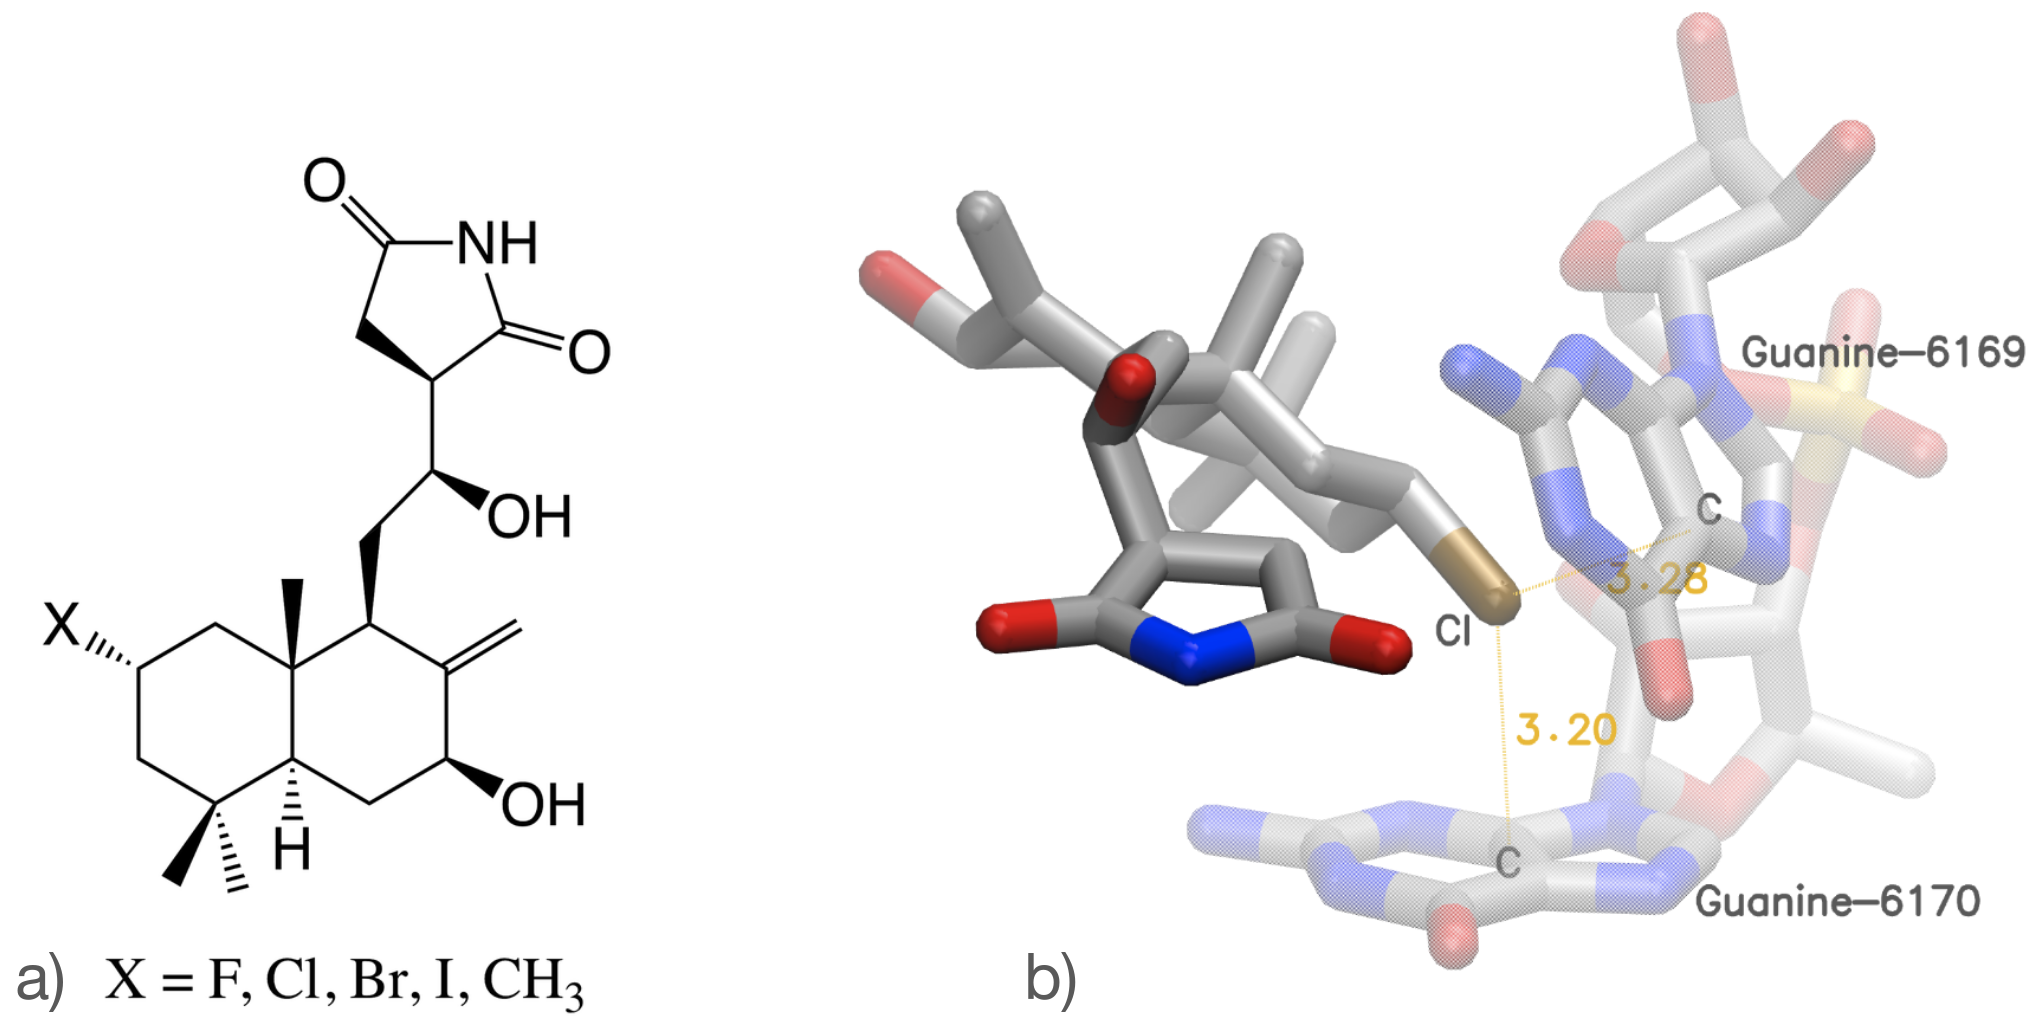
\includegraphics[scale=0.12]{combined.png}
  \caption{a) A series of substituted lissoclimides of different halogens.
    b) Geometry optimized model of CL and guanine nucleotides using the hybrid
    density functional TPSSh-D3.\autocite{Staroverov03JChemPhys119p12129,Grimme12ChemEurJ18p9955}
    Bond lengths are in Angstroms. Hydrogens were removed for clarity. Color codes
    for atoms are Cl = brown, N = blue, C = gray, O = red, and P = orange.\vspace{-11pt}}
  \label{fig:model}
\end{wrapfigure}

\textbf{Research Plan}

The halogen-$\pi$ interactions between the CL and ribosome were
studied based on a simplified model by K{\"o}nst \textit{et al.}\autocite{Konst2017}
I have performed preliminary work by improving upon this model and
varied the halogen moiety (X = F, Cl, Br, I, CH$_3$), see Fig. \ref{fig:model},
that showed binding energies increasing going down the halogen group. In addition,
the methylissoclimide surprisingly yielded a binding energy within 1
kcal/mol compared to iodolissoclimide. Dispersion interactions are expected
but, these remain to be intuitively understood. Hence, I will be spending time with
Prof. Filipp Furche attempting to capture and visualize the spontaneously induced
electronic attractions through analyzing the corresponding eigenvectors of the RPA
correlation energy. Lastly, I will work with Prof. Christopher Vanderwal to refine
and confirm the computational tool through the synthesis of the substituted lissoclimide
along with testing the drug's potency through \textit{in vitro} studies.

\textbf{Contribution to Doctoral Dissertation}

For my doctoral studies, I have envisioned my dissertation
to be focused on developing state-of-the-art approaches that accurately
describe NIs. We have concluded from our recent landmark publication that
RPA with its superior accuracy for NIs may safely replace MBPT for predictions
of NIs in most systems of chemical interest.\autocite{Nguyen20JChemTheoryComput16p2258}
With this research project, I will be able to apply diverse skills from
organic synthesis and theoretical chemistry to develop RPA based methods
that interpret NIs relevant for drug design.

\printbibliography

\end{document}
